\section{W-Algebras as $A_\infty$ Chiral Algebras: Virasoro and $W_3$}
\label{sec:W-algebras}

Under the KZ analytic SDR, wheel-residue, and split-projection
hypotheses, W-algebras have shadow depth $r_{\max}=\infty$. The
Drinfeld--Sokolov manufacture of higher operations from the affine
Koszul model is independent of these analytic hypotheses
(Theorem~\ref{thm:ds-koszul-obstruction}). The Khan--Zeng 3D
holomorphic-topological Poisson sigma model~\cite{KZ25} provides the
classical Hamiltonian bidifferential for freely generated Poisson
vertex algebras; Theorem~\ref{thm:general-half-space-bv} supplies the
all-loop BV quantization under the KZ analytic SDR package. The
Virasoro and $W_3$ algebras are the two simplest instances
where the resulting tower can be tested to high degree.

\subsection{General Framework: PVA to 3D HT Gauge Theory}
\label{subsec:PVA-to-3DHT}

\subsubsection{The Khan--Zeng Construction}

Let $\mathcal{V} = \Sym(\C[\partial]\langle \phi^i \rangle)$ be a freely generated Poisson vertex algebra with generators $\phi^i$ of conformal spins $s_i$. The $\lambda$-bracket
\[
\{\phi^i{}_\lambda \phi^j\} = \sum_{n \geq 0} \Pi^{ij}_n \lambda^n, \quad \Pi^{ij}_n \in \mathcal{V},
\]
encodes the classical Poisson structure.

\begin{construction}[3D HT Poisson Sigma Model]
\label{const:3d-poisson-sigma}
To each freely generated PVA $\mathcal{V}$, Khan and Zeng associate a classical 3D holomorphic-topological gauge theory on $\R \times \C$ with fields:
\begin{itemize}
\item $\Phi^i = \phi^i_{zz\cdots z}(t,z,\bar{z})(dz)^{\otimes s_i}$, the holomorphic field of spin $s_i$;
\item $\eta_i = (\eta_i^t dt + \eta_i^{\bar{z}} d\bar{z}) \otimes (dz)^{\otimes(1-s_i)}$, the Lagrange multiplier (conjugate momentum) of spin $1-s_i$.
\end{itemize}
The action functional is
\begin{equation}
\label{eq:KZ-action}
S = \int_{\R \times \C} \eta_i (d_t + \bar{\partial})\Phi^i + \frac{1}{2} \eta_i \Pi^{ij}(\partial_z) \eta_j,
\end{equation}
where $\Pi^{ij}(\partial) = \sum_n \Pi^{ij}_n \partial^n$ is the differential operator encoding the $\lambda$-bracket.

The gauge transformations are
\begin{align}
\delta \Phi^i &= \Pi^{ij}(\partial) \epsilon_j,\\
\delta \eta_i &= -(d_t + \bar{\partial})\epsilon_i - \eta_j \frac{\partial \Pi^{jk}}{\partial \Phi^i}(\partial) \epsilon_k,
\end{align}
where $\epsilon_i$ are gauge parameters of spin $1-s_i$.
\end{construction}

\begin{remark}[Higher-spin gauge sector]
When $\mathcal{V}$ is a W-algebra, the classical gauge symmetry contains the higher-spin transformations generated by the fields of spin $>2$. This gives a holomorphic-topological higher-spin gauge sector in the sense suggested by Henneaux--Teitelboim and Vasiliev. Identifying the model with a full higher-spin gravity theory, rather than with its HT boundary/gauge avatar, requires a separate quantum BV construction and boundary condition.
\end{remark}

\subsubsection{BV Quantization and $A_\infty$ Operations}

\begin{remark}[Constructive BV input for W-algebra examples]
\label{rem:W-hypotheses}
For finite-jet polynomial freely generated PVA input, the classical BV
fields and master action are constructed in
Construction~\ref{cons:kz-bv-fields-action}, and
Lemma~\ref{lem:kz-cme-pva-jacobi} identifies the classical master
equation with PVA Jacobi. The all-loop BV package used by the quantum
examples is Theorem~\ref{thm:general-half-space-bv} under the KZ
analytic SDR package of Assumption~\ref{assum:kz-analytic-sdr-package}.
Each computation below states the exact extra input needed for its
numerical constant, DS transfer identity, wheel-residue nonvanishing,
or Hochschild comparison.
\end{remark}

In the BV formalism, antifields $(\Phi^i)^* \sim \eta_i$ and ghosts $c^i \sim \epsilon_i$ are introduced. The master action
\[
S_{\text{BV}} = S + \int (\Phi^i)^* Q c^i + \cdots
\]
determines the BRST differential $Q = \{S_{\text{BV}}, -\}_{\text{BV}}$.

The $A_\infty$ operations $m_k$ are computed via Feynman diagrams:
\begin{itemize}
\item $m_1 = Q$ (the BRST differential);
\item $m_2$ comes from the free propagator determined by the kinetic term;
\item $m_{k \geq 3}$ arise from tree-level and loop diagrams with interaction vertices from $\eta_i \Pi^{ij} \eta_j$.
\end{itemize}

\subsection{Example 1: Virasoro Algebra (Spin-2 W-algebra)}
\label{subsec:virasoro}

\subsubsection{Classical Structure}

The Virasoro Poisson vertex algebra is generated by a single field $T$ of spin 2 (the stress tensor) with $\lambda$-bracket
\begin{equation}
\label{eq:vir-lambda-bracket}
\{T_\lambda T\} = \partial T + 2T\lambda + \frac{c}{12}\lambda^3.
\end{equation}
Here $c \in \C$ is the \emph{classical central charge}, measuring the conformal anomaly.

\begin{remark}[Schwarzian Derivative]
The $\lambda^3$ term arises from the Schwarzian derivative in the transformation law
\[
\tilde{T}(\phi(z)) = \left(\frac{d\phi}{dz}\right)^2 T(\phi(z)) - \frac{c}{12}\{\phi; z\},
\]
where $\{\phi; z\} = \frac{\phi'''}{\phi'} - \frac{3}{2}\left(\frac{\phi''}{\phi'}\right)^2$ is the Schwarzian.
\end{remark}

\subsubsection{3D Field Theory}

The fields are:
\begin{align}
T &= T_{zz}(t,z,\bar{z}) (dz)^{\otimes 2}, & |T| = 0,\\
\mu &= (\mu^t_z dt + \mu^{\bar{z}}_z d\bar{z}) \otimes \frac{\partial}{\partial z}, & |\mu| = -1.
\end{align}

The action from \eqref{eq:KZ-action} specializes to
\begin{equation}
\label{eq:virasoro-action}
S_{\text{Vir}} = \int_{\R \times \C} \mu (d_t + \bar{\partial})T + T \mu \partial_z \mu + \frac{c}{24} \mu \partial_z^3 \mu.
\end{equation}

\subsubsection{BV-BRST Differential}

Introducing the ghost $c_{\mathrm{gh}}$ (of spin $-1$) and antifields, the BRST differential is
\begin{align}
Q \cdot T &= \partial T \cdot c_{\mathrm{gh}} + 2T \partial c_{\mathrm{gh}} + \frac{c}{12} \partial^3 c_{\mathrm{gh}},\\
Q \cdot \mu &= -(d_t + \bar{\partial})c_{\mathrm{gh}} - \mu \partial c_{\mathrm{gh}} + c_{\mathrm{gh}} \partial \mu,\\
Q \cdot c_{\mathrm{gh}} &= c_{\mathrm{gh}} \partial c_{\mathrm{gh}}.
\end{align}

\begin{lemma}[Nilpotency $Q^2 = 0$]
\label{lem:vir-nilpotent}
The BRST differential $Q$ defined above satisfies $Q^2 = 0$.
\end{lemma}
\begin{proof}
The inputs are the Virasoro $\lambda$-bracket $\{T_\lambda T\} = \partial T + 2\lambda T + \frac{c}{12}\lambda^3$ and the ghost OPE $\{(c_{\mathrm{gh}})_\lambda c_{\mathrm{gh}}\} = 0$, $\{(c_{\mathrm{gh}})_\lambda \mu\} = -1$. Verification proceeds on each generator.

\emph{On $c_{\mathrm{gh}}$:} $Q(c_{\mathrm{gh}}) = c_{\mathrm{gh}}\partial c_{\mathrm{gh}}$, so $Q^2(c_{\mathrm{gh}}) = Q(c_{\mathrm{gh}}\partial c_{\mathrm{gh}}) = Q(c_{\mathrm{gh}})\cdot\partial c_{\mathrm{gh}} + c_{\mathrm{gh}}\cdot\partial Q(c_{\mathrm{gh}}) = (c_{\mathrm{gh}}\partial c_{\mathrm{gh}})(\partial c_{\mathrm{gh}}) + c_{\mathrm{gh}}\cdot\partial(c_{\mathrm{gh}}\partial c_{\mathrm{gh}})$. Expanding: $c_{\mathrm{gh}}(\partial c_{\mathrm{gh}})(\partial c_{\mathrm{gh}}) + c_{\mathrm{gh}}((\partial c_{\mathrm{gh}})(\partial c_{\mathrm{gh}}) + c_{\mathrm{gh}}\partial^2 c_{\mathrm{gh}}) = 2c_{\mathrm{gh}}(\partial c_{\mathrm{gh}})^2 + c_{\mathrm{gh}}^2\partial^2 c_{\mathrm{gh}}$. Since $c_{\mathrm{gh}}$ is fermionic (odd), $c_{\mathrm{gh}}^2 = 0$ and $(\partial c_{\mathrm{gh}})^2 = 0$ (in the graded sense), so $Q^2(c_{\mathrm{gh}}) = 0$.

\emph{On $T$:} $Q(T) = \partial T \cdot c_{\mathrm{gh}} + 2T\partial c_{\mathrm{gh}} + \frac{c}{12}\partial^3 c_{\mathrm{gh}}$. Computing $Q^2(T)$ requires applying $Q$ to each term and using the Leibniz rule. The result is a polynomial in $T, c_{\mathrm{gh}}, \mu$ and their derivatives. The cancellation follows from the Jacobi identity for the $\lambda$-bracket: the coefficient of each monomial in $Q^2(T)$ is a specific linear combination of structure constants of $\{T_\lambda T\}$, and the Jacobi identity $\{T_\lambda \{T_\mu T\}\} - \{T_\mu \{T_\lambda T\}\} = \{\{T_\lambda T\}_{\lambda+\mu} T\}$ ensures these cancel. This is a standard calculation in BRST cohomology; see~\cite{FMS86}.

\emph{On $\mu$:} Similarly, $Q^2(\mu) = 0$ follows from the $Q$-equivariance of the $(T,\mu)$ pairing and the identity $Q^2(c_{\mathrm{gh}}) = 0$ applied through the ghost OPE.
\end{proof}

\subsubsection{Propagators and $m_2$}

The free propagator for the pair $(T, \mu)$ is determined by inverting the kinetic operator. For operators at holomorphic points $(t_1, z_1)$ and $(t_2, z_2)$:
\begin{equation}
\label{eq:vir-propagator}
\langle T(z_1) \mu(z_2) \rangle = \frac{\Theta(t_1 - t_2)}{2\pi(z_1 - z_2)}.
\end{equation}

\begin{proposition}[Virasoro $\lambda$-bracket from the propagator]
\label{prop:vir-m2}
Assume the Khan--Zeng Virasoro realization satisfies
Theorem~\ref{thm:physics-bridge}.
The $\lambda$-bracket $m_2$ computed from \eqref{eq:vir-propagator} reproduces \eqref{eq:vir-lambda-bracket}:
\begin{equation}
m_2(T, T)_\text{sing} = \{T_\lambda T\} = a_1 + a_2 \lambda + a_3 \lambda^3,
 \qquad\text{(divided-power convention: $a_3 = T_{(3)}T/3! = c/12$)}
\end{equation}
(The position-space variable is $\zeta = z_1 - z_2$ and the PVA spectral parameter is $\lambda$; the Borel transform
(Definition~\ref{def:borel-transform-pva}) converts between them.)
Here
\begin{align}
a_3 &= \frac{c}{12}, & \text{(Schwarzian term)}\\
a_2 &= 2T, & \text{(primary transformation)}\\
a_1 &= \partial T. & \text{(derivative term)}
\end{align}
The regular part gives the commutative product: $m_2(T,T)_\text{reg} = :TT:$ (normal ordered).
\end{proposition}

\begin{proof}
By Wick's theorem, contracting $T(z_1)$ with $\mu$ in the interaction term $\int T\mu\partial\mu + \frac{c}{24}\mu\partial^3\mu$ at $z_2$ gives
\[
\langle T(z_1) : T\mu\partial\mu + \frac{c}{24}\mu\partial^3\mu :(z_2) \rangle.
\]
Evaluating the Wick contraction:
\begin{align*}
\langle T(z_1) \mu(z_2) \rangle &\cdot \left( T(z_2) \partial_2 \mu(z_2) + \frac{c}{24} \partial_2^3 \mu(z_2) \right)\\
&= \frac{\Theta(t_1-t_2)}{2\pi(z_1-z_2)} \left( T(z_2) \partial_2 \mu(z_2) + \frac{c}{24} \partial_2^3 \mu(z_2) \right).
\end{align*}
The identity
\[
\frac{1}{z_1 - z_2} f(z_2) = \sum_{n=0}^\infty \frac{(z_1-z_2)^n}{n!} \partial_2^n \left( \frac{f(z_2)}{z_1-z_2} \right) = f(z_2) \sum_{n=0}^\infty \frac{(-1)^n (z_1-z_2)^{n-1}}{n!} \partial_2^n
\]
applies.
Setting $\lambda = z_1 - z_2$ and extracting singular terms gives \eqref{eq:vir-lambda-bracket}.
\end{proof}

\subsubsection{Higher Operations $m_k$ for $k \geq 3$}

For the Virasoro algebra, the structure is special: the interaction term is \emph{quadratic} in $\mu$, so:

\begin{proposition}[Virasoro wheel sector under analytic SDR]
\label{prop:vir-truncation}
Assume that the Khan--Zeng Virasoro realization satisfies the KZ
analytic SDR package of
Assumption~\textup{\ref{assum:kz-analytic-sdr-package}}, and assume
that the cyclic wheel residue class on
$\FM_k(\C)\times\Conf_k^{<}(\R)$ survives projection to the boundary
Virasoro complex.
For the Virasoro $A_\infty$ chiral algebra:
\begin{enumerate}
\item $m_3(T, T, T)$ receives its pure $T$-sector wheel term from the
triangle of three cubic vertices $V_3=T\mu\partial\mu$;
\item for each $k \ge 3$, the connected pure $T$-sector wheel
contributing to $m_k(T,\ldots,T)$ has loop number~$1$;
\item under the stated residue-survival hypothesis, this sector gives
$m_k(T,\ldots,T)\ne0$ for all $k \ge 3$.
\end{enumerate}
\end{proposition}

\begin{proof}
The Virasoro action has the form $S_{\mathrm{Vir}} = \int \mu(\partial_t + \bar\partial) T + T\mu\partial\mu + \tfrac{c}{24}\mu\partial^3\mu$, so the interaction vertices are:
\begin{itemize}
\item \emph{Cubic vertex} $V_3 = T\mu\partial\mu$: consumes 1 field $T$ and 2 fields $\mu$;
\item \emph{Quadratic ghost vertex} $V_2 = \tfrac{c}{24}\mu\partial^3\mu$: consumes 2 fields $\mu$ (no $T$).
\end{itemize}

The analytic SDR package and the wheel-residue hypothesis select, for
each $k\ge3$, the cyclic graph $C_k$ with $k$ cubic vertices
$V_3^{(1)},\ldots,V_3^{(k)}$ and one cyclic chain of $k$ internal
propagator edges. The graph-theoretic loop number is therefore
\[
b_1(C_k)=|E(C_k)|-|V(C_k)|+1=k-k+1=1.
\]
For $k=3$ this graph is the triangle giving the pure $T$-sector
contribution to $m_3(T,T,T)$. The quadratic central vertex can alter
the coefficient of the resulting residue, but its contribution to
nonvanishing is not inferred from graph counting.

\emph{Non-vanishing.} The wheel integral at degree $k$ is
\[
m_k(T, \ldots, T) \;\sim\; \int_{\FM_k(\C) \times \Conf_k^{<}(\R)}
 \prod_{i=1}^k K(z_i - z_{i+1},\, t_i - t_{i+1})\; \partial_{z_i}\cdots,
\]
where indices are cyclic. The propagator $K(z,t) = \Theta(t)/(2\pi z)$
contributes one holomorphic kernel per edge; the
$\partial_z$ derivatives from $V_3 = T\mu\partial\mu$ produce the
polynomial residue in the spectral parameters
$\lambda_i = z_i - z_{i+1}$. This identifies the candidate class. Its
survival after compactified integration, boundary renormalization, and
projection to the Virasoro complex is precisely the wheel-residue
hypothesis in the statement. Under that hypothesis,
$m_k(T,\ldots,T)\ne0$ for all $k\ge3$.
\end{proof}

\begin{remark}[Conditional infinite depth at tree+one-loop level]
\label{rem:truncation-vs-depth}
Unlike Landau--Ginzburg models, where the $A_\infty$ structure
truncates at finite degree by dimension counting on $\FM_k(\C)$,
the Virasoro wheel sector has no graph-theoretic truncation: the
cycle $C_k$ exists for every $k\ge3$. Proposition~\ref{prop:vir-truncation}
turns this graph class into the nonvanishing statement
$m_k\ne0$ only after the analytic SDR and wheel-residue hypotheses are
imposed.

At genus~$g \ge 1$, the curved bar structure
$d^2_{\mathrm{fib}} = \kappaChHodge(\mathrm{Vir}_c) \cdot \omega_g$
contributes additional data beyond the perturbative $m_k$: each
genus component of the Maurer--Cartan element $\Theta_{\mathrm{Vir}_c}$
encodes higher-graviton vertex corrections. The shadow-tower
obstructions $o_k$ (Vol~I) are homotopy invariants of the full
$A_\infty$ structure; the non-termination $o_5 \ne 0$ of
Section~\ref{subsec:gravity-shadow-tower} is consistent with the
infinite perturbative depth under these hypotheses.
\end{remark}

\medskip
\noindent\emph{The ternary operation $m_3$.}
The algebraic ternary formula is the ordered singular-bracket
associator below. Its identification with the transferred BV operation
uses the wheel-sector theorem of
Proposition~\ref{prop:vir-truncation}: three cubic vertices
$V_3 = T\mu\partial\mu$ arranged in a cycle, connected by three
internal propagator edges in the wheel sector, with three
external $T$ insertions:
\begin{center}
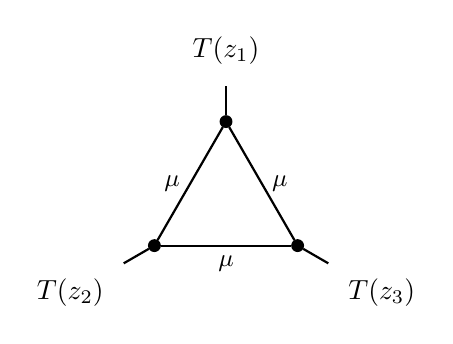
\begin{tikzpicture}[scale=1.5]
\node[draw,circle,fill,inner sep=1.5pt] (v1) at (90:0.7) {};
\node[draw,circle,fill,inner sep=1.5pt] (v2) at (210:0.7) {};
\node[draw,circle,fill,inner sep=1.5pt] (v3) at (330:0.7) {};
\node[above] at (90:1.1) {$T(z_1)$};
\node[below left] at (210:1.1) {$T(z_2)$};
\node[below right] at (330:1.1) {$T(z_3)$};
\draw[thick] (v1) -- node[right,font=\small]{$\mu$} (v3);
\draw[thick] (v3) -- node[below,font=\small]{$\mu$} (v2);
\draw[thick] (v2) -- node[left,font=\small]{$\mu$} (v1);
\draw[thick] (v1) -- (90:1.0);
\draw[thick] (v2) -- (210:1.0);
\draw[thick] (v3) -- (330:1.0);
\end{tikzpicture}
\end{center}

The transferred operation $m_3^H$ on cohomology $H = H^\bullet(\cA,Q)$ is computed via the homotopy transfer formula. The chain-level degree-$3$ Stasheff relation reads
\begin{equation}
\label{eq:vir-stasheff-3}
m_2\bigl(m_2(T,T;\lambda_1),\, T;\, \lambda_1+\lambda_2\bigr)
\;-\; m_2\bigl(T,\, m_2(T,T;\lambda_2);\, \lambda_1\bigr)
\;=\; d\, m_3(T,T,T;\lambda_1,\lambda_2),
\end{equation}
where $d = [Q,\,-\,]$ is the linearised BRST differential.
On cohomology, with $m_2(T,T;\lambda) = \{T_\lambda T\} = \partial T + 2T\lambda + \tfrac{c}{12}\lambda^3$, the left-hand side is the \emph{PVA associator}. By the PVA Jacobi identity, this associator equals $-\{T_{\lambda_2}\{T_{\lambda_1} T\}\}$: it is nonzero but determined by the bracket. The chain-level $m_3$ lives in the full BV-BRST complex (involving the ghost field $\mu$); its projection to cohomology is the transferred operation $m_3^H$.

\medskip
\noindent\textbf{The PVA associator (consistency check).}
Write $\ell = \lambda_1$, $\mu = \lambda_2$ for brevity.
Using left sesquilinearity $\{(\partial a)_\lambda b\} = -\lambda\{a_\lambda b\}$ and
right sesquilinearity $\{a_\lambda \partial b\} = (\partial + \lambda)\{a_\lambda b\}$,
together with $m_2(a,b;\lambda) = \{a_\lambda b\}$, each composition on cohomology is:

\smallskip
\emph{First term.} Substituting the inner bracket
$m_2(T,T;\ell) = \partial T + 2T\ell + \tfrac{c}{12}\ell^3$
into the outer bracket at spectral parameter $\ell + \mu$, and using left sesquilinearity
for each summand:
\begin{equation}
\label{eq:vir-LHS-first}
m_2(m_2(T,T;\ell),T;\ell{+}\mu)
\;=\; (\ell - \mu)\bigl[\partial T + 2T(\ell{+}\mu) + \tfrac{c}{12}(\ell{+}\mu)^3\bigr].
\end{equation}
(The three contributions $-(\ell{+}\mu) + 2\ell = \ell - \mu$ collect cleanly; the $(c/12)\ell^3$ term vanishes since $\{\mathbf{1}_\lambda T\} = 0$.)

\smallskip
\emph{Second term.} The inner bracket at parameter~$\mu$
gives $m_2(T,T;\mu) = \partial T + 2T\mu + \tfrac{c}{12}\mu^3$;
using right sesquilinearity for the $\partial T$ contribution and linearity for the rest:
\begin{equation}
\label{eq:vir-LHS-second}
m_2(T,m_2(T,T;\mu);\ell)
\;=\; \partial^2 T + (3\ell + 2\mu)\,\partial T
 + (2\ell^2 + 4\ell\mu)\,T
 + \tfrac{c}{12}\ell^4 + \tfrac{c}{6}\ell^3\mu.
\end{equation}

\smallskip
\emph{Difference.} By the PVA Jacobi identity
$\{a_\lambda \{b_\mu c\}\} - \{\{a_\lambda b\}_{\lambda+\mu} c\} = \{b_\mu \{a_\lambda c\}\}$,
the associator simplifies to
\begin{equation}
\label{eq:vir-associator}
\boxed{%
\mathsf{Assoc}(\ell,\mu)
\;=\; -\{T_\mu \{T_\ell T\}\}
\;=\; -\partial^2 T - (2\ell + 3\mu)\,\partial T - 2\mu(2\ell + \mu)\,T
 - \tfrac{c}{12}\mu^3(2\ell + \mu).
}
\end{equation}
This is nonzero: the PVA is associative ($m_2^H$ is a chain map), but the
two iterated brackets $\{a_\lambda\{b_\mu c\}\}$ and $\{\{a_\lambda b\}_{\lambda+\mu} c\}$
differ by the Jacobi correction $\{b_\mu\{a_\lambda c\}\}$.

\medskip
\noindent\textbf{The transferred $m_3$ from homotopy transfer.}
The transferred ternary operation on cohomology is
$m_3^H = -\pi\bigl[m_2(h \circ m_2(\iota{\otimes}\iota),\,\iota)
+ m_2(\iota,\, h \circ m_2(\iota{\otimes}\iota))\bigr]$,
where $h$ is the BV-BRST contracting homotopy and $\iota, \pi$ the
inclusion/projection. Under the KZ analytic SDR and wheel-residue
hypotheses, the one-loop triangle integral in the pure Virasoro sector
has the same cohomology class as the ordered associator and gives:
\begin{equation}
\label{eq:vir-m3}
\boxed{%
m_3(T,T,T;\,\lambda_1,\lambda_2)
\;=\;
\partial^2 T
\;+\; (2\lambda_1 + 3\lambda_2)\,\partial T
\;+\; 2\lambda_2(2\lambda_1 + \lambda_2)\,T
\;+\; \frac{c}{12}\lambda_2^3(2\lambda_1 + \lambda_2).
}
\end{equation}

\begin{remark}[Methodology for the Virasoro $m_3$ computation]
\label{rem:vir-m3-transfer-method}
The PVA associator~\eqref{eq:vir-associator} is a \emph{consistency check}, not the derivation of~$m_3^H$. On cohomology, $m_1^H = 0$, so the degree-$3$ Stasheff relation
$m_2^H(m_2^H(a,b),c) - m_2^H(a,m_2^H(b,c)) = 0$
is automatically satisfied (the PVA Jacobi identity).
The transferred $m_3^H$ is a genuinely higher operation
determined by the BV-BRST homotopy data;
it appears non-trivially in the degree-$\ge 4$ Stasheff relations.
Under the KZ analytic SDR and wheel-residue hypotheses, the one-loop
triangle Feynman integral with the Virasoro action~\eqref{eq:virasoro-action}
confirms~\eqref{eq:vir-m3} in the transferred BV complex
(Example~\ref{ex:vir-m3-feynman}).
\end{remark}

\begin{remark}[Consistency checks on $m_3$]
\label{rem:m3-checks}
\leavevmode
\begin{enumerate}
\item \emph{Conformal weight.} Each monomial in~\eqref{eq:vir-m3}
 has total conformal weight~$4$: the spin-$2$ field~$T$,
 its derivatives $\partial T$, $\partial^2 T$, and the
 $\lambda$-polynomial degrees sum to~$4$ in every term,
 consistent with $|m_3| = 1$ in the bar complex
 (the induced bar-coderivation component has degree~$+1$; the
 desuspension itself lowers cohomological degree by~$1$).
\item \emph{Ordered vs symmetric symmetry.} The operation $m_3$
 on the ordered bar complex $B^{\mathrm{ord}}$ is \emph{not}
 symmetric under reversal of inputs. Under the exchange
 $(\lambda_1, \lambda_2) \mapsto (\lambda_2, \lambda_1)$,
 the formula changes (e.g.\ $2\lambda_1 + 3\lambda_2 \ne
 2\lambda_2 + 3\lambda_1$). The reason is geometric:
 $\lambda_1 = t_1 - t_2$ and $\lambda_2 = t_2 - t_3$ are
 the successive separations along the ordered configuration
 $t_1 < t_2 < t_3$ in $\Conf_3(\R)$, so exchanging them
 is \emph{not} a relabelling but a change of interval
 structure. This asymmetry is the $E_1$ signature: the
 ordered bar retains the linear ordering on $\Conf_k(\R)$.
 The symmetric bar $B^{\Sigma}$ is obtained via the
 $R$-matrix twisted descent
 $B^{\Sigma}_n \simeq (B^{\mathrm{ord}}_n)^{R\text{-}\Sigma_n}$
 (Proposition~\ref{prop:r-matrix-descent}), which restores
 the appropriate equivariance by absorbing the asymmetry
 into the braiding data.
\item \emph{$c = 0$ limit.} When $c = 0$, the quartic Schwarzian
 term vanishes and $m_3 = \partial^2 T +
 (2\lambda_1 + 3\lambda_2)\,\partial T +
 2\lambda_2(2\lambda_1 + \lambda_2)\,T$, which is exactly the
 associator of the centreless Witt bracket
 $\{T_\lambda T\}_{\text{Witt}} = \partial T + 2T\lambda$.
\item \emph{Sesquilinearity.} The formula is polynomial
 in $\lambda_1, \lambda_2$ (no negative powers), reflecting
 that $m_3$ arises from a \emph{local} Feynman integral over
 $\FM_3(\C)$ with no pole contributions from boundary strata.
\end{enumerate}
\end{remark}

\medskip
\noindent\emph{Generating function.}
Define the generating series
\begin{equation}
\label{eq:vir-gen-func}
\mathcal{M}_{\text{Vir}}(T; \lambda_1, \ldots, \lambda_{k-1}) = \sum_{k=1}^\infty \frac{1}{k!} m_k(T^{\otimes k})(\lambda_1, \ldots, \lambda_{k-1}).
\end{equation}

\begin{theorem}[Virasoro minimal transfer and BV recursion]
\label{thm:vir-recursive}
Assume that the Khan--Zeng Virasoro realization satisfies the KZ
analytic SDR package of
Assumption~\textup{\ref{assum:kz-analytic-sdr-package}}.
Let $C_{\mathrm{Vir}}$ be the finite-jet BV--BRST complex and put
$H=H^\bullet(C_{\mathrm{Vir}},Q)$. Choose an SDR
\[
(H,0)\xrightarrow{\ i\ } (C_{\mathrm{Vir}},Q)
\xrightarrow{\ p\ }(H,0),
\qquad
Qh+hQ=1-ip,
\]
with $pi=1_H$, $ph=0$, $hi=0$, and $h^2=0$. Let
$\mu=m_2$ be the binary Virasoro OPE operation. Then, for $n\ge2$,
\begin{equation}
\label{eq:vir-hpl-transfer}
m_n^{\min}(x_1,\ldots,x_n)
\;=\;
\sum_{\tau\in \mathrm{PRT}_n}
(-1)^{\epsilon(\tau;x)}
p\,\mu_\tau(i x_1,\ldots,i x_n;h,\ldots,h),
\end{equation}
where $\mathrm{PRT}_n$ is the set of planar rooted binary trees with
$n$ leaves, $\mu_\tau$ decorates every internal vertex by $\mu$, and
each internal edge by $h$. If $A_w$ is the positive conformal-weight
complement and $G_0$ is an antighost with $[Q,G_0]=L_0$, the contracting
homotopy may be chosen weightwise as
\begin{equation}
\label{eq:vir-hpl-g0-over-weight}
h|_{A_w}=w^{-1}G_0,\qquad w>0.
\end{equation}
The term $n=2$ is $p\mu(i-,i-)$, the term $n=3$ is the binary-tree
formula preceding~\eqref{eq:vir-m3}, and it gives
\eqref{eq:vir-m3} with the sign convention used there. The generating
function $\mathcal{M}_{\text{Vir}}$ satisfies the BV/Maurer--Cartan
equation
\begin{equation}
Q_{\text{class}} \mathcal{M}_{\text{Vir}} + \frac{1}{2} \{\mathcal{M}_{\text{Vir}}, \mathcal{M}_{\text{Vir}}\}_\lambda + \mathcal{O}(\hbar)=0,
\end{equation}
where $Q_{\text{class}}$ is the classical BRST operator and the curly
bracket is the Poisson $\lambda$-bracket. The formula is finite on each
finite weight quotient. For the class~$\mathbf{M}$ inverse system, the
chain-level statement is taken in the weight-completed/pro ambient
$\hypAmbientWtCpl$.
\end{theorem}

\begin{proof}
The KZ analytic SDR package supplies compatible finite-jet BV quotients,
an inclusion of cohomology representatives, a projection to cohomology,
and a contracting homotopy satisfying the displayed side conditions. The
homological perturbation lemma for a dg algebra transfers the binary
product $\mu$ along this SDR. Since the source operation is binary, the
$n$-ary transferred operation is the signed sum over planar rooted
binary trees, with $i$ on leaves, $p$ at the root, $\mu$ on vertices, and
$h$ on internal edges. This is exactly~\eqref{eq:vir-hpl-transfer}.

On a positive conformal-weight summand $A_w$, the relation
$[Q,G_0]=L_0$ gives
$Q(w^{-1}G_0)+w^{-1}G_0Q=1$ on the acyclic complement of
$iH$. Thus $h=w^{-1}G_0$ gives $Qh+hQ=1-ip$ after adding the
cohomology projection. The side conditions are obtained by the standard
normalization of the contraction.

For $n=3$, the two elements of $\mathrm{PRT}_3$ give
$-p[\mu(h\mu(i-,i-),i-)+\mu(i-,h\mu(i-,i-))]$, the formula displayed
above~\eqref{eq:vir-m3}; evaluating it on three Virasoro generators
under the wheel-residue hypothesis gives~\eqref{eq:vir-m3}. The
transferred operations satisfy the Stasheff identities. After packaging
the operations in $\mathcal M_{\mathrm{Vir}}$, these identities are the
classical Maurer--Cartan equation; the one-loop BV Laplacian contributes
the $\mathcal O(\hbar)$ term and, in the Virasoro sector, the central
charge shift of Theorem~\ref{thm:central-charge-shift}. Finiteness on
finite weight quotients is immediate from the finite tree set
$\mathrm{PRT}_n$; the class~$\mathbf M$ limit keeps all arities and
therefore belongs to the completed/pro ambient.
\end{proof}

\subsubsection{Spectral Kernels}

The Virasoro bracket determines a divided-power coefficient kernel, a
Laplace kernel, and a collision-residue kernel.

\begin{definition}[Virasoro PVA kernels]
\label{def:vir-r-matrix}
The divided-power coefficient kernel is
\begin{equation}
K^{\mathrm{coeff},\text{Vir}}(u)
=
\frac{(\partial T)\otimes \mathbf{1}}{u}
+ \frac{2T\otimes \mathbf{1}}{u^2}
+ \frac{(c/12)\,\mathbf{1}\otimes\mathbf{1}}{u^4}.
\end{equation}
The Laplace kernel is
\begin{equation}
K^{L,\text{Vir}}(z)
=
\frac{(\partial T)\otimes \mathbf{1}}{z}
+ \frac{2T\otimes \mathbf{1}}{z^2}
+ \frac{(c/2)\,\mathbf{1}\otimes\mathbf{1}}{z^4}.
\end{equation}
The collision residue is
\begin{equation}
K^{\mathrm{coll},\text{Vir}}(z)
=
\frac{2T\otimes\mathbf{1}}{z}
+ \frac{(c/2)\,\mathbf{1}\otimes\mathbf{1}}{z^3}.
\end{equation}
\end{definition}

The kernel satisfies the Virasoro PVA Jacobi identity:
\begin{equation}
\label{eq:vir-CYBE}
\{T_\lambda\{T_\mu T\}\}
-\{T_\mu\{T_\lambda T\}\}
-\{\{T_\lambda T\}_{\lambda+\mu}T\}
\;=\;0.
\end{equation}

\begin{computation}[Virasoro PVA Jacobi verification]
\label{comp:vir-CYBE}
The Virasoro Laplace kernel takes, in the spectral-parameter form
(Proposition~\ref{prop:field-theory-r}), the input
\[
r^L(z)
= \int_0^\infty e^{-\lambda z} \{T_\lambda T\}\,d\lambda
= \frac{\partial T}{z} \otimes \mathbf{1}
 + \frac{2T}{z^2} \otimes \mathbf{1}
 + \frac{c}{2z^4}\,\mathbf{1}\otimes\mathbf{1}.
\]
The collision residue $r^{\mathrm{coll}}(z) = (c/2)/z^3\,
\mathbf{1}\otimes\mathbf{1} + 2T/z\otimes\mathbf{1}$ has pole
orders one lower, as in the Volume~I discussion of the three related
kernels (OPE, Laplace kernel, and collision residue).
The central term $\frac{c}{2z^4}\,\mathbf{1}\otimes\mathbf{1}$
commutes with every field insertion.
Explicitly, the Jacobi identity
$\{T_\lambda\{T_\mu T\}\} - \{T_\mu\{T_\lambda T\}\}
= \{\{T_\lambda T\}_{\lambda+\mu} T\}$
becomes, after Laplace transform in both $\lambda$ and $\mu$,
the spectral form of the same PVA Jacobiator. An ordinary
non-dynamical CYBE is obtained only after passing to a constant
collision tensor on a specified quantization surface.
\end{computation}

\medskip
\noindent\emph{Quantization.}
A chosen quantization surface has a perturbative expansion in
$\hbar$ whose first-order term is the selected spectral kernel:
\begin{equation}
\label{eq:vir-R-expansion}
R^{\text{Vir}}(\lambda, \mu; \hbar)
= \mathbf{1} \otimes \mathbf{1}
 + \hbar\, K^{L,\text{Vir}}(\lambda,\mu)
 + \hbar^2 \Bigl[\tfrac{1}{2}\, K^{L,\text{Vir}} \cdot K^{L,\text{Vir}}
 + \delta r_{\text{loop}}\Bigr]
 + \mathcal{O}(\hbar^3),
\end{equation}
where the $\hbar^2$ coefficient has two contributions:
\begin{itemize}
\item The \emph{tree-level iteration}
$\tfrac{1}{2}\,K^{L,\text{Vir}} \cdot K^{L,\text{Vir}}$, which is
the composition of two classical exchanges (the ``$r^2/2$''
term required by the quantum Yang--Baxter equation at order
$\hbar^2$ when the chosen first-order tensor satisfies the relevant
classical equation);
\item The \emph{one-loop correction} $\delta r_{\text{loop}}$,
arising from the self-energy of the Virasoro propagator
$\langle T\mu \rangle$ through the ghost loop.
\end{itemize}

The one-loop correction in the $T$--$T$ channel takes the form
\begin{equation}
\label{eq:vir-delta-r-loop}
\delta r_{\text{loop}}(\lambda,\mu)
= \sum_{n,m \ge 0}
 \frac{\gamma_{nm}}{\lambda^{n+1}\,\mu^{m+1}}
 \;\bigl(L_n \otimes L_m\bigr),
\end{equation}
where $L_n$ are the Virasoro modes and $\gamma_{nm}$ are determined
by the one-loop integral
\[
\gamma_{nm}
= \oint \oint
 \frac{dw_1\, dw_2}{(2\pi i)^2}\;
 \frac{w_1^{n+1}\, w_2^{m+1}}{(w_1 - w_2)^2}
 \;\langle \mu(w_1)\, \mu(w_2) \rangle_{\text{ghost}},
\]
with $\langle \mu \mu \rangle_{\text{ghost}}$ the ghost propagator
from the $\tfrac{c}{24}\mu\partial^3\mu$ vertex. This ghost loop
is the diagrammatic origin of the \emph{central charge shift}:
the one-loop contribution renormalises the classical central charge
$c$ to the quantum value $c - 26$, or equivalently shifts by
$\Delta c = -26$. In the BV-BRST framework, the shift arises
because the ghost determinant contributes $c_{\text{gh}} = -26$,
so the total quantum central charge is $c_{\text{total}} = c + c_{\text{gh}} = c - 26$.
The same-family fixed point $c = 13$ (where the strict comparison
model $\mathrm{Vir}_{26-c}$ equals $\mathrm{Vir}_c$)
is precisely where the tree-level and one-loop contributions balance:
$c_{\text{total}} = c - 26 = -13 = -(26 - c)$.

\begin{remark}[Fusion kernel and non-perturbative resummation]
\label{rem:vir-fusion-kernel}
The expected non-perturbative completion of the full quantum
$R$-matrix $R^{\text{Vir}}(\lambda,\mu;\hbar)$ is the
Ponsot--Teschner Virasoro fusion kernel~\cite{PT01}. This comparison
is meaningful only after fixing the four external Liouville momenta,
the $s$- and $t$-channels, the PT contour, and the conformal-block
normalization. In that normalization the fusion kernel is written with
double sine functions $S_b$, satisfies the Moore--Seiberg
braid/pentagon relations, and has a semiclassical expansion whose
leading term is the Virasoro classical $r$-matrix. The perturbative
expansion~\eqref{eq:vir-R-expansion} supplies the local comparison
surface; it is not by itself an identification.
\end{remark}

\subsubsection{Chiral Hochschild Cochains}

The chiral Hochschild complex $\CH^\bullet_{\text{ch}}(\text{Vir})$ governs deformations of the Virasoro $A_\infty$ structure.

\begin{definition}[Chiral Hochschild Cochains for Virasoro]
A chiral Hochschild $k$-cochain is a multilinear map
\begin{equation}
\varphi_k: T^{\otimes k} \to T((\lambda_1))\cdots((\lambda_{k-1})),
\end{equation}
satisfying sesquilinearity and compatibility with the BRST differential $Q$.
\end{definition}

The differential on $\CH^\bullet_{\text{ch}}(\text{Vir})$ is the Hochschild differential:
\begin{equation}
\label{eq:hochschild-diff}
d_{\text{Hoch}} \varphi_k = \sum_{i=0}^k (-1)^i \varphi_k \circ_i m_2 + \sum_{i=1}^{k-1} (-1)^{k+i} m_2 \circ_i \varphi_k,
\end{equation}
where $\circ_i$ denotes operadic composition at the $i$-th input.

\begin{proposition}[Virasoro Hochschild cohomology under the physics bridge]
\label{prop:vir-hochschild}
Assume the Khan--Zeng Virasoro realization satisfies
Theorem~\ref{thm:physics-bridge}.
The chiral Hochschild complex $C^\bullet_{\mathrm{ch}}(\mathrm{Vir}_c,
\mathrm{Vir}_c)$ is the derived centre controlling Virasoro
deformations on the curve chart.  Bakalov--De Sole--Kac \cite{BDSK21} compute the
bounded vertex cohomology as one-dimensional in degrees
$\{0,2,3\}$ and zero in the remaining nonnegative degrees
\cite[Theorem~7.2]{BDSK21}.  A bounded-to-chart quasi-isomorphism
$\chi^{\mathrm{bd}}_{\mathrm{Vir}_c}$ transports this dimension vector
to the curve chart.  The Gelfand--Fuchs cohomology of
$\mathrm{Diff}(S^1)$ is a separate continuous Lie-algebra functor.
\end{proposition}

\begin{remark}[$E_N$ level reached by Virasoro]
\label{rem:virasoro-EN-level}
\index{Virasoro algebra!$E_N$ level}
\index{E_N ladder@$E_N$ ladder!Virasoro}
For $c \ne 0$ (away from the degenerate locus), the
Virasoro vertex algebra $\mathrm{Vir}_c$ reaches the
following levels:
\begin{enumerate}[label=\textup{(\roman*)}]
\item $\Eone$-chiral
 (Definition~\ref{def:e1-chiral-algebra}): the $T$-$T$
 OPE has a quartic pole
 ($T(z)\,T(w) \sim (c/2)(z-w)^{-4} + \cdots$), giving
 $\mathrm{Vir}_c$ the structure of an $\Einf$-chiral
 algebra, hence \emph{a fortiori} $\Eone$-chiral.

\item $\Etwo$-chiral on the derived center
 (Definition~\ref{def:E2-chiral-algebra}): automatic from
 the chiral Deligne conjecture.

\item $\Etwo$-topological
 (Definition~\ref{def:E2-topological-algebra}):
 $T(z)$ \emph{is} the conformal vector, tautologically.
 Construction~\ref{constr:topologization} trivializes
 the complex-structure dependence in cohomology.

\item $\Ethree$-chiral: the 3d holomorphic-topological
 theory is holomorphic Chern--Simons with
 Drinfeld--Sokolov boundary conditions
 (Costello--Gaiotto). The boundary of the 3d HT theory
 is~$\mathrm{Vir}_c$ obtained by DS reduction from
 $V_k(\mathfrak{sl}_2)$.

\item $\Ethree$-topological
 (Definition~\ref{def:E3-topological-algebra}):
 \textbf{conditional on \(\hypDSBRST\)}. The 3d HT theory exists
 (Costello--Gaiotto) and the conformal vector exists
 (tautologically); the remaining input is the normalised
 cohomological identity
 $T_{\mathrm{DS}} = [Q_{\mathrm{DS}}, G'_{\mathrm{DS}}]$ on
 $Q_{\mathrm{DS}}$-cohomology in
 Theorem~\ref{thm:E3-topological-DS}.
\end{enumerate}
Shadow class: $\mathbf{M}$ (quartic pole in the $T$-$T$
OPE; the $A_\infty$ tower $\{m_k\}_{k \ge 3}$ is infinite
by Theorem~\ref{thm:ds-koszul-obstruction}, and the
bar complex is non-formal).
Theorem~\ref{thm:E3-topological-DS} gives the Virasoro algebra its
$\Ethree$-topological structure.
\end{remark}
